\section{Comparison}
\label{section:comparison}

\par Now a comparison between the theoretical analysis and the experimental analysis results of the gain is done.
 
%colocar graficos do gain theoretical vs experimental
\begin{figure}[ht]
\centering
\begin{subfigure}{.5\textwidth}
  \centering
  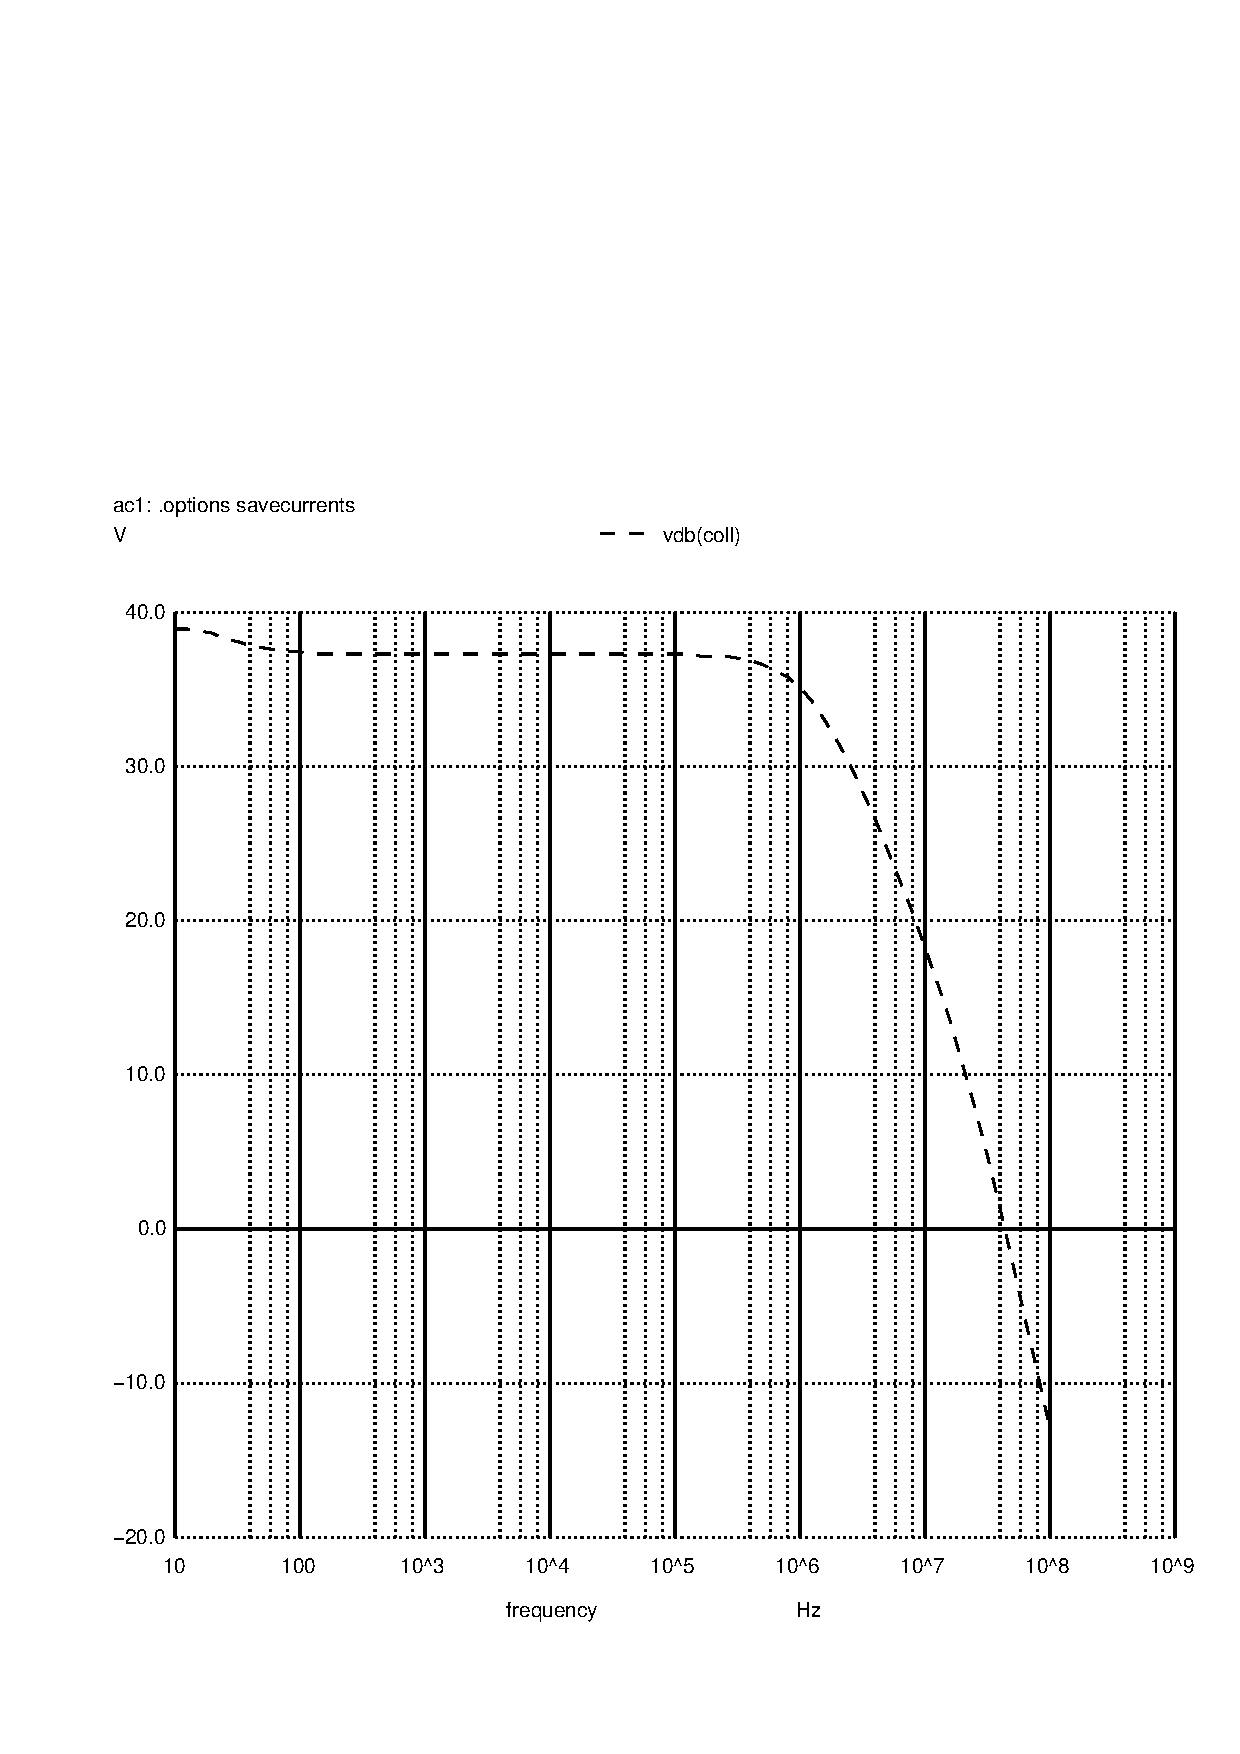
\includegraphics[width=.75\linewidth]{vo1f.pdf}
  \caption{Input Voltage}
  \label{fig:sim4}
\end{subfigure}%
\begin{subfigure}{.5\textwidth}
  \centering
  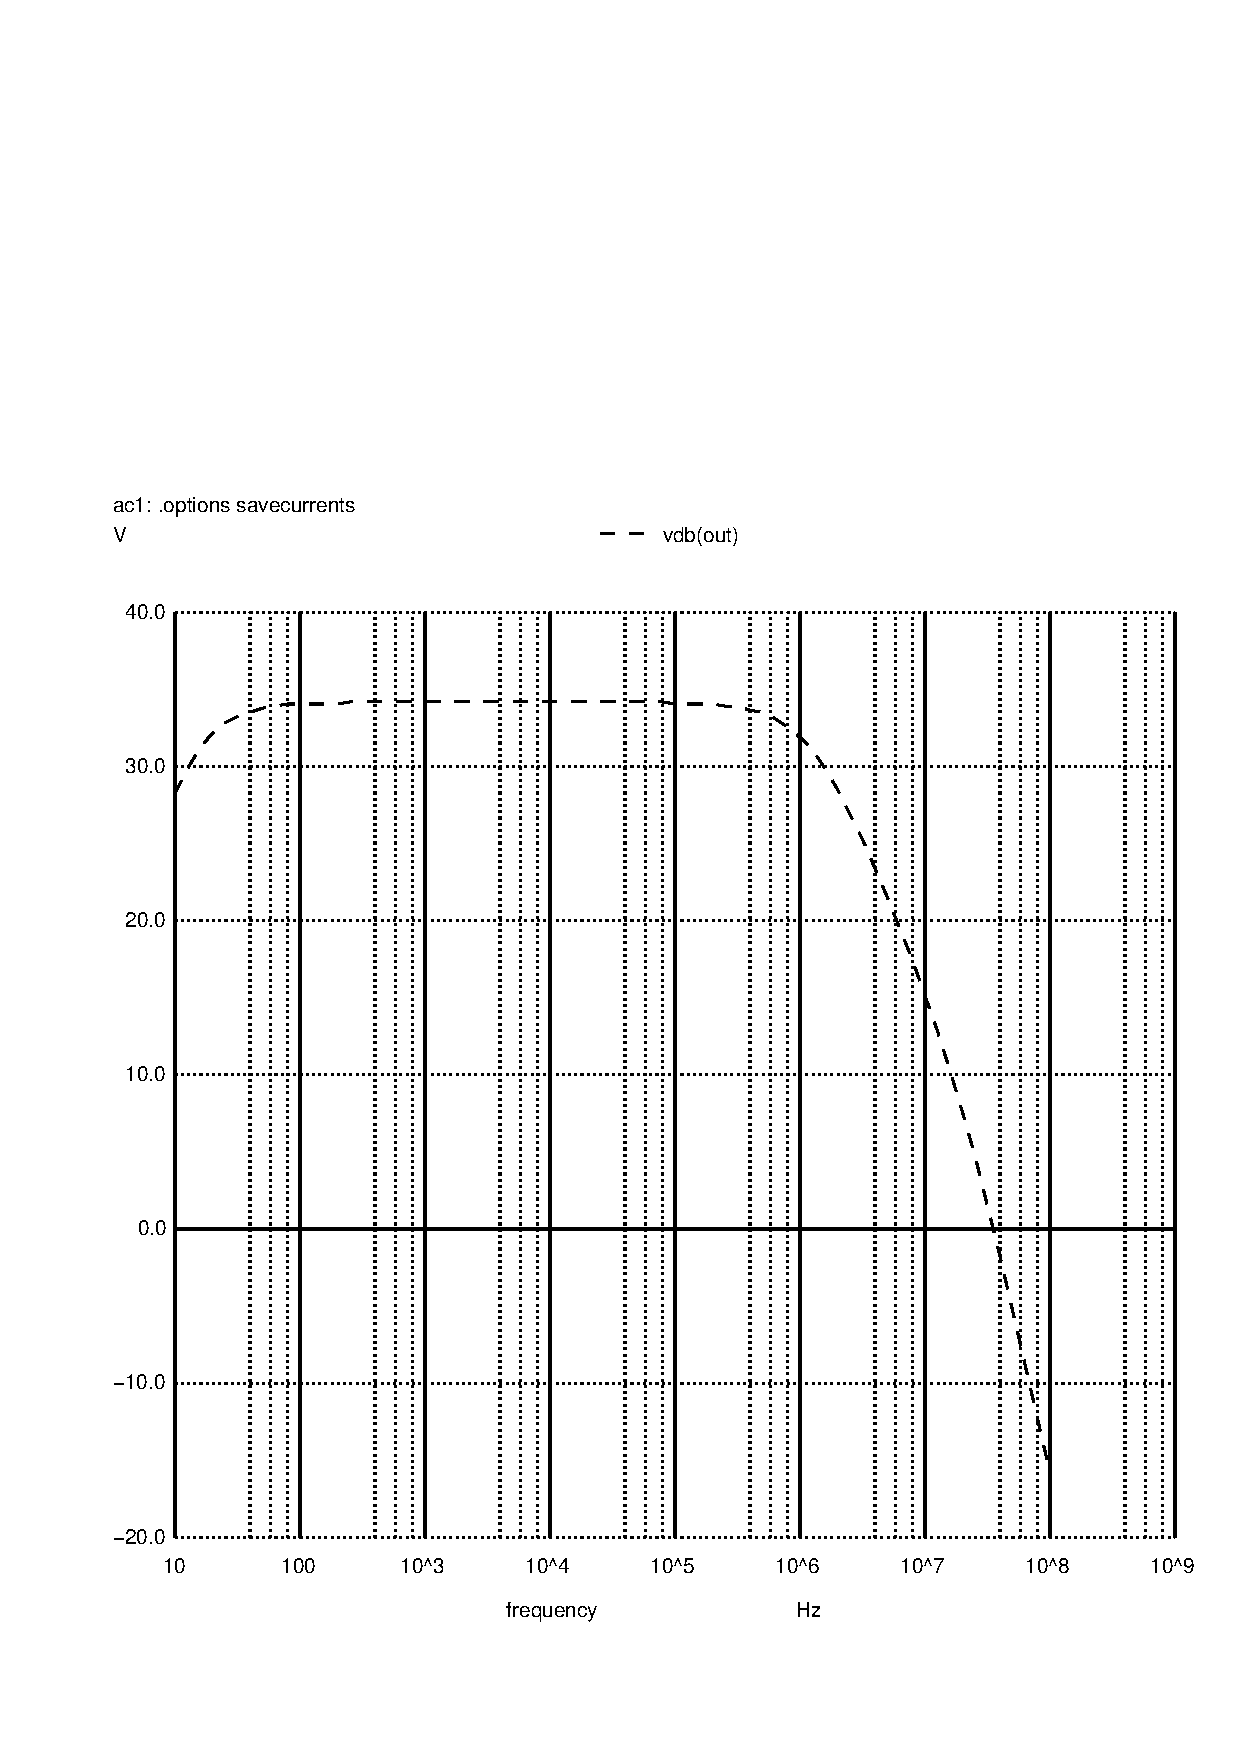
\includegraphics[width=.75\linewidth]{vo2f.pdf}
  \caption{Output voltage}
  \label{fig:sim5}
\end{subfigure}
\end{figure}

\par As we can see the graphics are pretty similar, which means that our theoretical model is a good approximation to the real running of an audio amplifier. Furthermore we can compare the values which we are studying and trying to improve: maximum gain and bandwidth and also a comparison between the operating point values is going to be made. The values are shown in the table below.

TABLEEEEEEEEEEEEE

\par As we can  

\par As we can see there are some errors associated with the theoretical model when compared to the experimental results, especially for the values of the voltage in the nodes.
Nosso
********************************
TEKAs



In the Ngspice table, the only parameters in comparison are $@q1[ib]$, $@q1[ic]$, $@q1[ie]$, $base$, $coll$ and $emit$.
\par As one may observe, some discrepancies in the voltage values are noticeable. Nevertheless, the values of the currents flowing are are within reasonable intervals of similarity. Therefore, the gain computed in Octave should not be severely affected by this. It is important to highlight that the theoretical gain expression is dependent on the value of the current $I_{C}$ because of the incremental parameter $g_{m}$. 

\par Aditionally, the gain, bandwidth and cut off frequency results were also computed. As predicted, the voltage gain in the theoretical approach is greater than in the Ngspice computation. Moreover, since we do not have the theoretical high cut frequency, we can only compare the results for the low cut frequency, which are very similar as far as the order of magnitude is concerned. For this reason, as the bandwidth is the subtraction between high and low cut frequencies, it should not be compared.









